%%%%%%%%%%%%%%%%%%%%%%%%%%%%%%%%%%%%%%%%%%%%%%%%%%%%%%%%%%%%%%%%%%%%%%%%%%%%%%%%
%2345678901234567890123456789012345678901234567890123456789012345678901234567890
%        1         2         3         4         5         6         7         8

\documentclass[11pt, onecolumn, compsoc, letterpaper]{article}
%\usepackage{times}

% Subfiles package
%\usepackage{subfiles}

% Usual setup packages
\usepackage{listings} % For including source code with highlighting
\usepackage{hyperref} % For better hyper-link integration
\usepackage[bottom]{footmisc} % places footnotes at page bottom

% Packages for verbatim text blocks
\usepackage{alltt} % Package for including math in verbatim text
\usepackage{fancyvrb}

% Packages for math symbols and other mathey things
\usepackage{amsthm}
\usepackage{amsmath}
\usepackage{amsfonts}
\usepackage{amssymb}

% Packages for including pseudo-code
\usepackage{algorithmicx}
\usepackage{algorithm}
\usepackage{algpseudocode}

% Packages that handle tables, figures and other floats
\usepackage{tabularx}
\usepackage{multirow}
\usepackage{float} % To make floats movable
\usepackage{subcaption}
\usepackage[table]{xcolor}

% Packages for drawing graphs, FSMs, etc.
\usepackage{pgf}
\usepackage{tikz}
\usetikzlibrary{shapes,arrows,calc,fit,positioning,shapes.symbols,shapes.callouts,patterns,automata,matrix}

% Remove red boxes around refs
\hypersetup{
    colorlinks,
    citecolor=black,
    filecolor=black,
    linkcolor=black,
    urlcolor=blue
}

% Squeeze whitespace
\usepackage{geometry} % to change the page dimensions
\usepackage[compact]{titlesec}
\usepackage{titling}

\setlength{\parskip}{0pt}
\setlength{\parsep}{0pt}
\setlength{\headsep}{0pt}
\setlength{\topskip}{0pt}
\setlength{\topmargin}{0pt}
\setlength{\topsep}{0pt}
\setlength{\partopsep}{0pt}

\titlespacing{\section}{0pt}{*3}{*3}
\titlespacing{\subsection}{0pt}{*2}{*2}
\titlespacing{\subsubsection}{0pt}{*1}{*1}

\renewcommand{\arraystretch}{1.2}
\setlength{\droptitle}{-2cm}

% ------------------------------ CUSTOM MACROS ------------------------------------
% Nice little macro for adding a comment box. Include incrementing comment numbers.
\newcounter{comcount}
\setcounter{comcount}{0}
\newcommand{\mycomment}[1]
{
\refstepcounter{comcount}
\smallskip\noindent\fbox{\parbox{\linewidth}{\emph{Comment \arabic{comcount}} : \small{#1}}} 
}

% - Math
\DeclareMathOperator*{\argmin}{\arg\!\min\>}
\newcommand{\amin}[1]{\underset{#1}\argmin}
\DeclareMathOperator*{\argmax}{\arg\!\min\>}
\newcommand{\amax}[1]{\underset{#1}\argmax}

\newcommand{\abs}[1]{\lvert#1\rvert}
\newcommand{\norm}[1]{\lVert#1\rVert}
\newcommand{\D}[2][t]{\frac{d#2}{d#1}}
\newcommand{\PD}[2][t]{\frac{\partial #2}{\partial #1}}
\newcommand{\V}[1]{\mathbf{#1}}
\newcommand{\sig}{\mathcal{S}}
\newcommand{\ceil}[1]{\lceil#1\rceil}
\newcommand{\xm}{x_{\hat{m}}}

% To keep footnotes on the same page are reference
\interfootnotelinepenalty=10000
\raggedbottom

\begin{document}
\title{Ph.D. Thesis Proposal}
\author{Anshul Kanakia}

\maketitle

\section{Introduction}
Many social, biological and physical systems can be represented as swarm systems. From modeling human societal interaction and population dynamics to insect colonies and great animal herd migrations, from cellular automata to distributed network systems and even the interconnected computing devices that form the internet---which is the collective sum of human knowledge today---can be viewed as swarm intelligence. \emph{Swarm Robotics} \cite{Sahin2005} is a branch of swarm intelligence applied to physical multi-agent systems (MAS) to leverage the advantage of producing emergent, complex behavior from individually simplistic agents and rules. This has led to novel approaches in the design and analysis of MAS and the algorithms associated with them \cite{Brambilla2013}.

Swarm systems have many benefits over traditional, centralized robot systems. The robots used in swarm applications are generally many orders of magnitude smaller (\emph{cm} vs.~\emph{m}, \emph{grams} vs.~\emph{kg}) and simpler in design ($<10$ vs.~$100$s of actuators) than conventional robots, while being much greater in number ($10^2$ to $10^{<<23}$). Also, most swarm systems are homogeneous---robots with identical software/hardware are used to complete the assigned task. This makes swarm systems easily scalable while simultaneously keeping manufacturing and maintenance costs of the hardware low. Though, perhaps their greatest advantage is system stability and robustness to error. Most swarm systems consist of small, relatively simple robots that are only capable of limited and noisy sensing, communication and actuation. This means that while no single robot alone is capable of performing the task assigned, the system as a whole is resilient to individual unit errors and is capable of completing the task \cite{Winfield2005}.

Swarm robotics has tackled a vast array of MAS problems in the past two decades. It's corpus ranges from self-organization, self-assembly, pattern formation, and aggregation to foraging, coordinated movement (such as flocking and schooling), and group surveillance. Readers are directed to \cite{Bayindir2007} and the references therein for further information on any of these topics. 

Performing collaborative tasks is a vast sub-field of study in swarm robotics and a considerable work has been done to understand and model such scenarios, particularly by Agassounon, Ijspeert and Martinoli using the well known stick-pulling experiments \cite{Martinoli1995, Martinoli1999b, Agassounon2001, Ijspeert2001, Agassounon2002}. Collaborative tasks using MAS extend to a variety of potential real-world applications such as oil-spill containment, firefighting (particularly large forest fires), object transport, and group surveillance and, as such, form a significant subclass of problems to study and analyze. Am important question that has so far remained unanswered when attempting collaborative tasks is how many agents are required to complete a given task of a certain size and how are they recruited? It is often assumed that all robots are pre-programmed to form groups of a particular size beforehand or that the task requires an \emph{exact} number of robots to complete successfully---a number that is known beforehand. 

\begin{figure}[!tb]
	\centering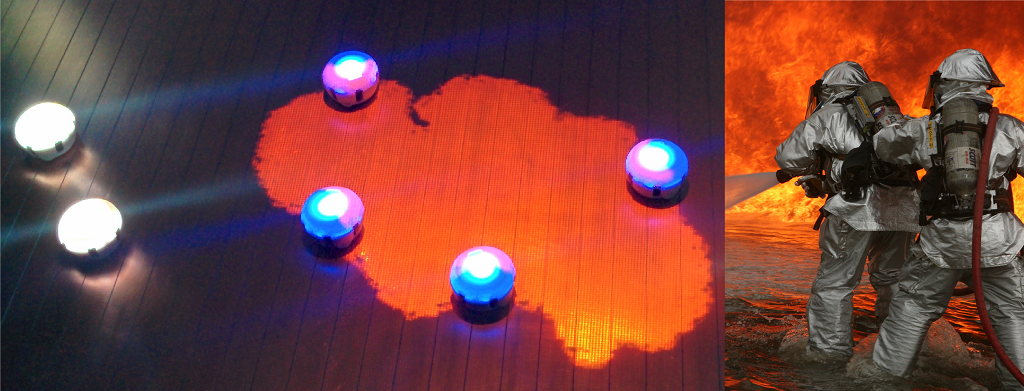
\includegraphics[width=\textwidth]{../assets/dropletfire.png}
	\centering\caption{The \emph{Droplet} swarm robots running a fire containment experiment inspired by a real forest firefighting scenario (copyright, \emph{Creative Commons}).}\label{fig:dropletfire}
\end{figure}

But what about tasks that are dynamic in nature such as fighting forest fires? In such cases it is impractical and often impossible to know beforehand, exactly how many agents are required for successful completion. More importantly, the benefit of larger teams of agents for such collaborative tasks increases non-linearly with team size, e.g. Where 1-5 robots may be incapable of lifting a heavy object, 6-7 will be able to lift and move it successfully. I define such tasks with non-linear increase in system utility with increasing team sizes as ``Concurrent Benefit'' tasks. It is for such situations that I propose a novel methodology for estimating group sizes in a distributed fashion, as described by my thesis statement below.

\section{Thesis Statement}
\begin{quote}
My goal is to provide a fully distributed methodology for estimating appropriate team sizes required to complete concurrent benefit tasks using minimal communication in a MAS setting. I will analyze this methodology using tools from optimization and game theory to provide theorems on overall efficiency and resultant group behavior while supporting these claims using numerical and physics-based simulations as well as real robot experiments.
\end{quote}

This approach to solving the problem of group size estimation differs from existing approaches in swarm robotics that are often constrained by the inherent physical and memory limitations of small, simplistic robots. Applications of MAS to real-world scenarios is lacking today because many of the existing swarm robot platforms are exceedingly simplistic and are not capable of handling complex tasks such as rough terrain traversal, carrying heavy objects, long-distance communication, etc. that are required for tackling actual situations. While the focus of my research is not on hardware design, I aspire to develop a more adaptable and mathematically rigorous solution for group size estimation and recruitment that is oblivious to the physical restrictions of a robotic platform and works in almost all MAS settings. The only assumptions I make reasonably are that whatever hardware my algorithms run on is capable (however imperfectly) of the four basic requirements of robotics; actuation, sensing, communication and computation.

\section{Proposed Work}
In this section I will outline my proposed research work, focusing heavily on two main aspects of my thesis statement; modeling and analysis of swarm systems and my specific work on team size estimation, in that order.

\subsection{Consistent Modeling Methodology for Swarm Robotics}
The first issue any swarm robotics researcher faces is a distinct lack of established modeling methodology in the field.  This is why review papers is swarm robotics as recent as 2007 \cite{Bayindir2007} still cite modeling as an open research topic for the field. In order to make swarms an alternative engineering approach---in which robustness emerges despite predictable, individual failure---we require formal tools that allow us to predict and verify the resulting complex behavior. Developing such tools goes hand-in-hand with investigating novel hardware, simulation tools \cite{Michel1998}, and tracking tools \cite{correlliros06,lochmatter08} that ease conducting large numbers of experiments with large numbers of robots. Analyzing swarm dynamics on a higher abstraction level allows us to explore the design space much faster, but also to use parameter analysis and numerical methods for optimization and verification.

\begin{figure}[!htb]
	\centering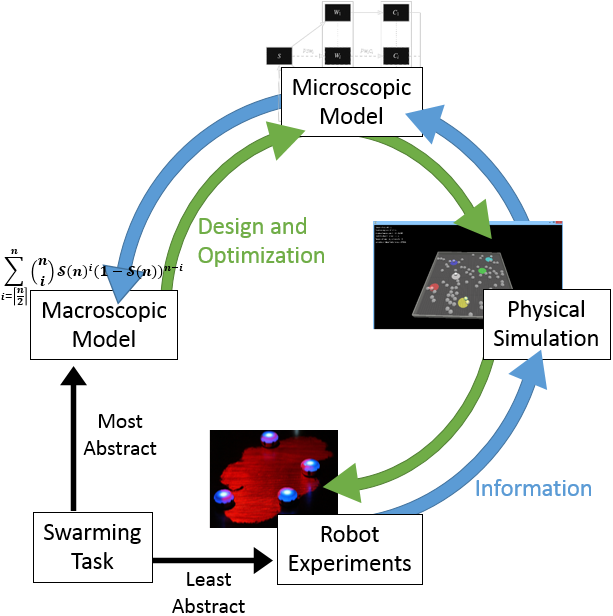
\includegraphics[width=.75\textwidth]{../assets/ssmodel.png}
	\centering\caption{The closed loop optimization model for swarm systems. Real robot experiments and physical simulations provide paramter dicovery and information while mathematical models are used to opitimize these parameters for maximizing swarm utility.}\label{fig:ssmodel}
\end{figure}

For this purpose, I propose a closed loop system as seen in Fig.~\ref{fig:ssmodel}. Setting up the required swarming task as a real physical experiment or physical simulation allows us to discover and measure the different free parameters in the system. We then use these variables in lower resolution models (micro-level) as well as in the development of mathematical models (macro-level) for our system. These more abstract models allow us to rapidly experiment with system parameters and optimize them. We can then use these optimized parameters back in the real physical experiments to improve the desired behavior of the system and repeat the cycle till the desired level of accuracy and satisfaction of model behavior is achieved. A closed loop modeling methodology also allows us to identify and optimize important system parameters as described in \cite{Correll2006a,Correll2008}.

\subsubsection{\emph{Droplet} Hardware and Simulation Platform}
An important step in any modeling process is validation by comparing model results to real experiment data. Given the relatively abstract approach we have seen so far for designing models of robot swarms, this step is made even more crucial. The micro and macro-models in swarm robotics have conventionally been designed using observed phenomena from other processes seen in biological and chemical systems and adapted to fit the swarming task being studied. Many swarm algorithms show emergent behavior where the observation of complex properties at the system level cannot be trivially inferred from studying the individual agent behavior. The generalizations and simplifications made in the robot controller design when developing the micro and macro-models can suppress the interesting emergent properties seen in real physical systems.

\begin{figure}[!ht]
\begin{subfigure}{.5\textwidth}
\centering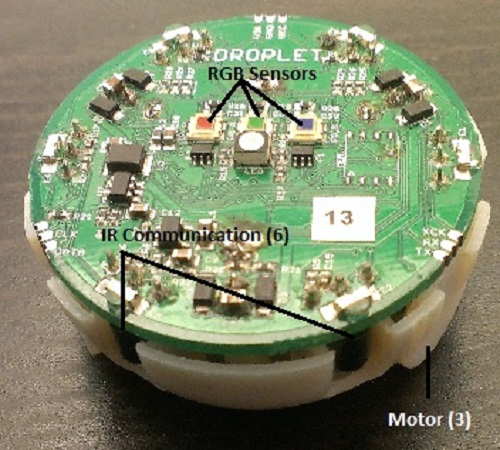
\includegraphics[width=6.5cm]{../assets/droplettop.jpg}
\centering\caption{The Droplet robot.}\label{fig:dropletrbt}
\end{subfigure}~
\begin{subfigure}{.5\textwidth}
\centering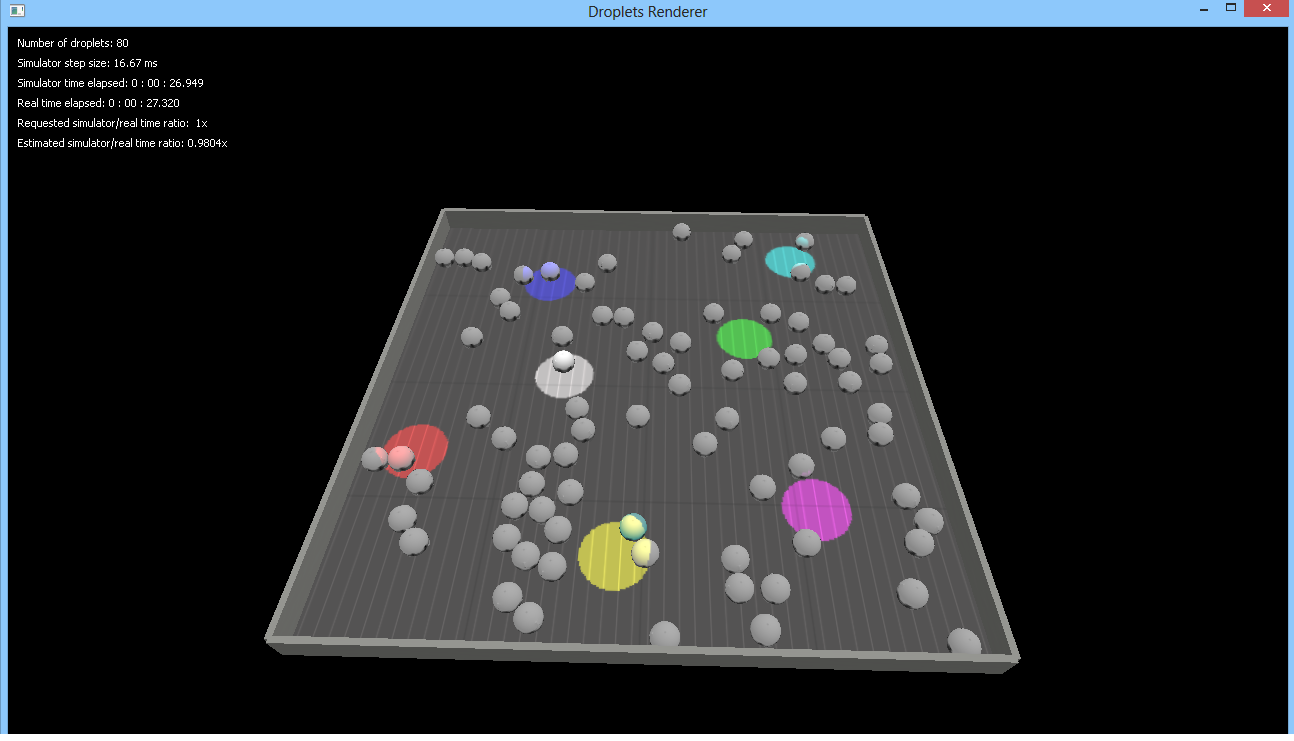
\includegraphics[width=6.5cm]{../assets/dsim.png}
\centering\caption{The Droplet simulator.}\label{fig:dropletsim}
\end{subfigure}
\caption{}
\end{figure}

I have thus spent a considerable amount of my time as a graduate student helping build and design a 1000 agent swarm platform and accompanying simulator called the \emph{Droplet} swarm robot platform\footnote{This project is open source and is funded by NSF Grant \#$1150223$. The code is available in these GitHub repositories,
\begin{itemize}
\item Droplet Swarm Robot Platform: \url{https://github.com/correlllab/cu-droplet}
\item Droplet Swarm Robot Simulator: \url{https://github.com/correlllab/cu-droplet-sim}
\end{itemize}}. 
Each individual Droplet robot runs on an ATMEL XMega 128 A3U processor and is capable of RGB sensing and omnidirectional motion and IR communication. The Droplet swarm robot simulator uses a physics engine (\emph{Bullet} physics) for realistic simulation of the Droplets and has proved to be an invaluable rapid prototyping test-bed for my research. While not directly related to my proposed work, I have co-authored a conference publication  about the hardware motion sub-system of the Droplets \cite{Klingner2014} and have played a major role in the platform's development over the years.

I will incorporate all these modeling aspects that make up different parts of the closed loop controller for swarm systems into a tutorial journal paper. Having a consistent methodology for analyzing swarm systems is paramount in standardizing the algorithm development process in this field, which has progressed using only ad-hoc and phenomenological approaches till now.

\subsection{Collaboration Model using a Sigmoid Threshold Function}
\begin{figure}[!htb]
\begin{subfigure}{0.5\textwidth}
\centering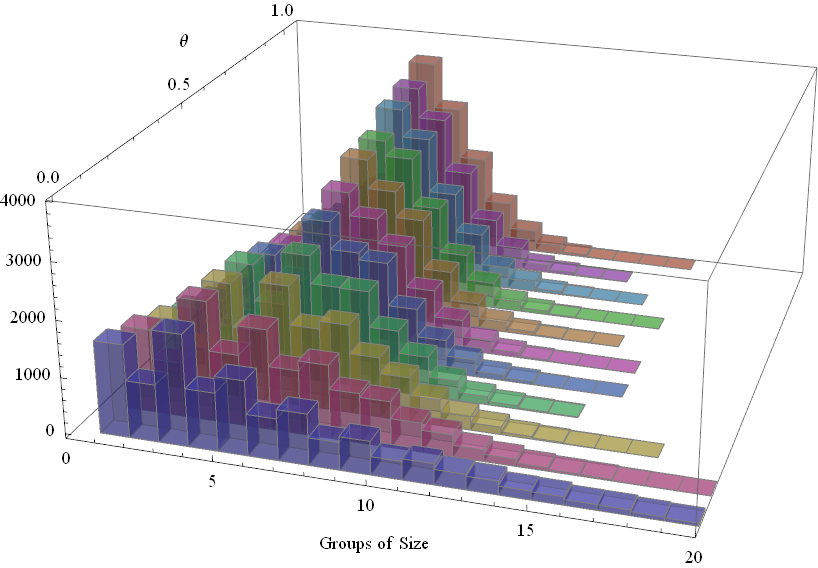
\includegraphics[width=1.0\textwidth]{../assets/collabratesweep4.png}
\centering\caption{$\tau = 4$}\label{fig:collabsweep4}
\end{subfigure}~
\begin{subfigure}{0.5\textwidth}
\centering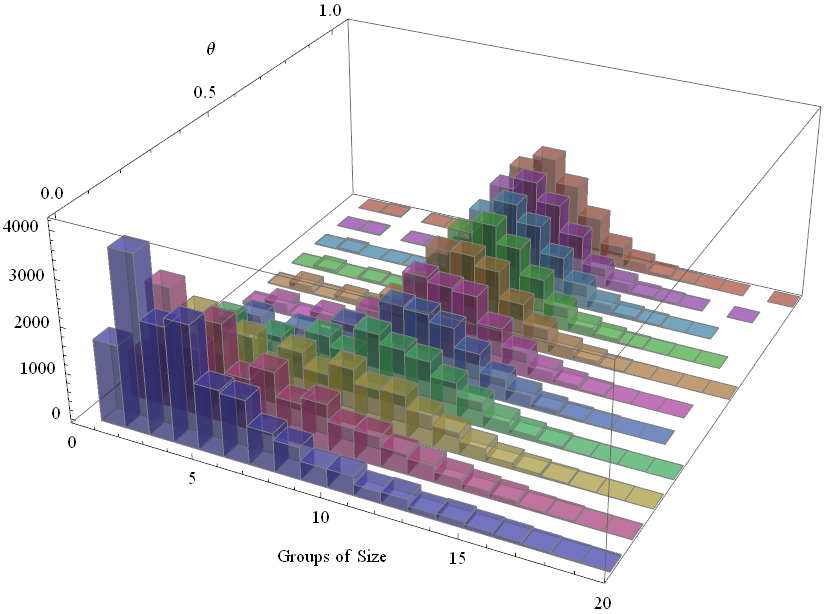
\includegraphics[width=1.0\textwidth]{../assets/collabratesweep8.png}
\centering\caption{$\tau = 8$}\label{fig:collabsweep8}
\end{subfigure}
\begin{subfigure}{0.5\textwidth}
\centering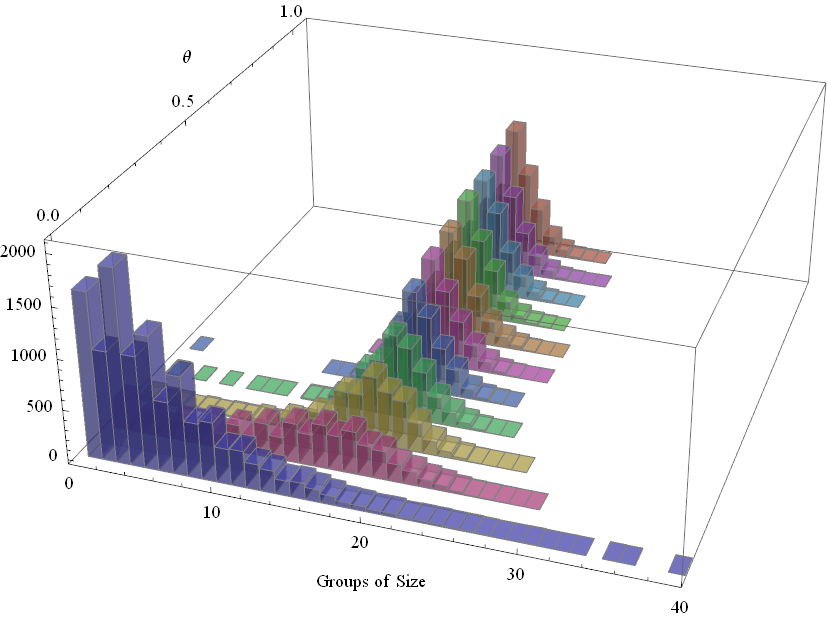
\includegraphics[width=1.0\textwidth]{../assets/collabratesweep16.png}
\centering\caption{$\tau = 16$}\label{fig:collabsweep16}
\end{subfigure}~
\begin{subfigure}{0.5\textwidth}
\centering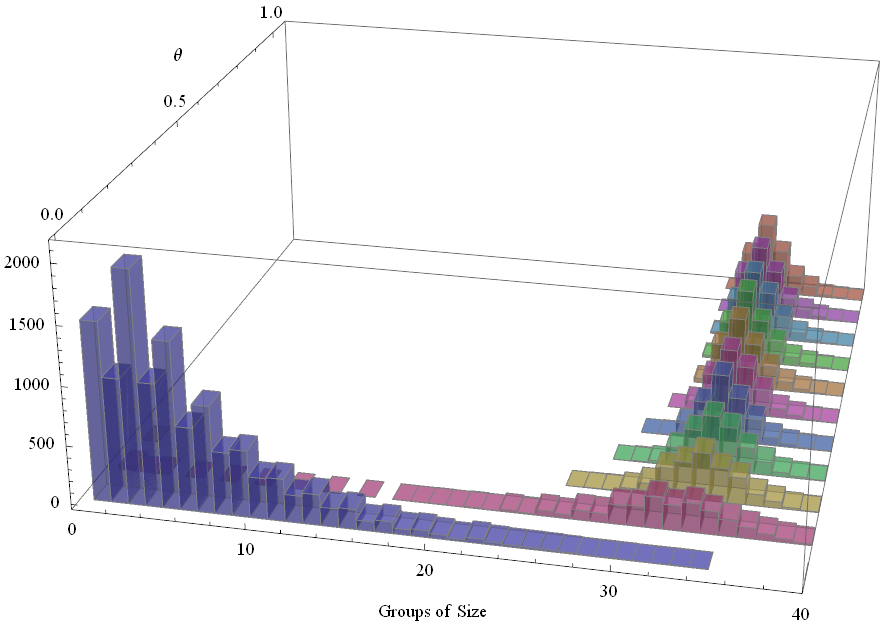
\includegraphics[width=1.0\textwidth]{../assets/collabratesweep32.png}
\centering\caption{$\tau = 32$}\label{fig:collabsweep32}
\end{subfigure}
\caption{Histograms of resulting team sizes for various values of $\tau$ and $\theta$ with one hundred robots and one collaboration site.}\label{fig:collabsweep}
\end{figure}

Returning to the second half of my thesis statement, I would like to do an in-depth study of team size recruitment for concurrent benefit tasks.  Recruiting robots to collaboratively solve a task is a canonical problem in robotics \cite{Gerkey2004}. Other research groups have spent considerable time analyzing \cite{Martinoli2004, Martinoli1995, Lerman2001} collaborative tasks using exact team sizes. I wish to generalize this work to account for tasks with unknown or approximate prior required team sizes. I have already studied how sigmoid threshold functions can be used as a voting mechanism in collaboration problems for achieving this goal. We can tune the logistic function, as seen below, using two parameters $\tau$ and $\theta$ which map to the mean and variance for desired team sizes, respectively.

\begin{equation}
	\sig(\xm) = \frac{1}{1 + e^{\theta(\tau - x)}}
\end{equation}\label{eq:sigmoid}

My DARS 2014 publication (Best paper award), analyzed this task allocation model using probability theory and a finite state machine (FSM) controller to drive individual agents' decisions on whether to begin a collaborative task with a group or to wait until more agents to join the group. The probability that a group of agents of size-$n$ will decide to collaborate is given by,

\begin{equation}
	P(n) = \sum\limits_{i={n/2}}^{n}\binom{n}{i}\sig(\tau, \theta, n)^{i}\left(1 - \sig(\tau, \theta, n)\right)^{n - i}
\end{equation}\label{eq:cdf}

An interesting feature of this equation is that by setting all other unknowns, $\tau$, $n$ and $P(n)$ we can solve for a $\theta$, the group size variance parameter, that provides probabilistic guarantees for groups of size $\leq n$ forming with probability = $P(n)$. This allows us to find a appropriately accurate $\theta$ for a range of desired group sizes. While this math was presented in the paper, the broad conclusion I just described was left out for space requirements and further analysis. It will be included in my dissertation and the journal article I plan on writing about sigmoid threshold based task allocation. 

\begin{figure}[!htb]
\centering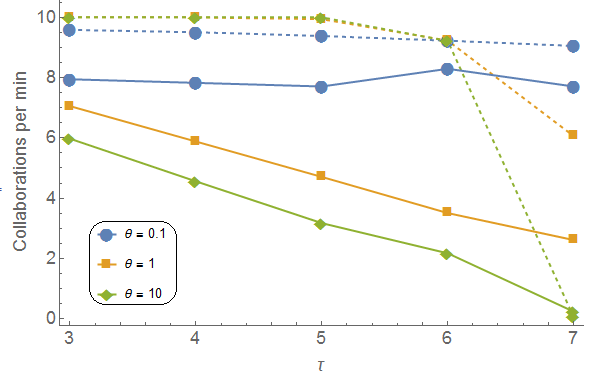
\includegraphics[width=0.55\textwidth]{../assets/realsimexpnew.png}
\caption{The solid lines show collaborations per min, over 15min, for a group of 6 real robots as the desired group size is varied from 3 to 7 and the slope of $\sig$ is varied between $0.1, 1$ and $10$. The dashed lines indicate simulation results with the same parameters.\label{fig:expdat} }
\end{figure}

We ran also Gillespie simulations \cite{Gillespie1976, Gillespie1977} (see Fig.~\ref{fig:collabsweep}) as well as real robot experiments using the Droplets to verify our findings(see Fig.~\ref{fig:expdat}). The data in Fig.~\ref{fig:expdat} shows a clear mismatch between real robot and simulation experiments. This is, in part, due to the fact an important step in the proposed algorithm involves having agents make an estimate of their current group size (this is the term $\xm$ in eq.~\ref{eq:sigmoid}). Noisy/Imperfect communication between agents in the real robot setting consistently led to underestimates in group size which is why we see a considerable drop in collaboration rate. This problem can be mitigated using higher variance values for team size and as well as Bayesian inferencing techniques to get a better estimate of the actual number of robots sharing a site, using prior knowledge of the environment. I wish to study this problem further and address it in the journal article I mentioned earlier.

\subsection{Application of Game Theory to MAS}
A novel tool that is becoming increasingly applicable to the field of swarm robotics is \emph{Game Theory} \cite{GivigiJr2006, Panait2005}. Being formally introduced in John von Neumann's seminal work, "Zur Theorie der Gesellschaftsspiele" (On Theory of Games and Strategy) in 1928, game theory has since been applied to a vast array of fields such as economics, biology and, more recently, computer science to study the mathematical models of conflict and cooperation between intelligent rational decision-makers. The direct analogy of  a rational \emph{player} in a game to a robot in a swarm or agent in an MAS setting makes the use of game theory techniques natural in these settings to analyze overall system behavior.

There is a subclass of games known as \emph{Global Games} \cite{Carlsson1993, Morris2001} which I think lines up very well with my current task allocation model. Global games are those where agents receive possibly correlated signals about the fundamental underlying state of the system and make independent decisions based on their noisy belief of this signal. See \cite{Morris2001} and the references therein for more details. This global games setup can be mapped to a realistic MAS scenario where agents have to sense and impending collaborative task (such as a forest fire) in the environment using their noisy sensors and independently make estimates on what an appropriate group size should be to tackle this task. 

One of the possible outcomes of representing the collaboration model as a global game is that a fundamental result of the equilibrium conditions on global games can be applied to this MAS setting. This result claims that, making certain assumptions about the underlying correlated signal and noise distributions, equilibrium for a global game is achieved when every player uses a threshold policy when making their independent yes/no decisions on whether or not to collaborate. Analyzing the equilibrium conditions associated with this game and understanding their influence in a real robot setting is a very interesting problem and could provide a fundamental result for the best collaboration policy to use for concurrent benefit tasks. This result could show that my sigmoid threshold function is an optimal control policy for such tasks. I am currently in the process of writing a conference paper about it. This analysis will form the crux of my dissertation.

\section{Conclusion}
In conclusion, I would like to re-iterate my proposed work before my defense. I would like to write one journal article that discusses closed loop-optimization for multi-agent systems utilizing different abstraction levels from real hardware experiments to macroscopic mathematical models. I will explain the benefits of propagating system-level information from less abstract to more abstract models and use that information to drive design and optimization of MAS using numerical simulation and other viable techniques. 

Further, I would also like to use this modeling methodology to study, in-depth, the problem of team size estimation using minimal communication for tasks which share the property of concurrent benefit, i.e. where system level utility increases non-linearly with increasing team sizes. I am in the process of writing one conference paper about results from global games, a subclass of game theory, on concurrent benefit tasks and I would like to write on journal article that consolidates all my findings on this MAS collaboration model. 

\section{Published and In-Progress Work}
\begin{enumerate}
	\item Klingner, J., Kanakia, A., Farrow, N., Reishus, D., \& Correll, N. ``A stick-slip omnidirectional powertrain for low-cost swarm robotics: Mechanism, calibration, and control.'' Intelligent Robots and Systems (IROS 2014), 2014 IEEE/RSJ International Conference on. IEEE, 2014.
	\item Kanakia, A., \& Correll, N. ``A Response Threshold Sigmoid Function Model for Swarm Robot Collaboration.'' Distributed and Autonomous Robotic Systems (DARS 2014), \emph{Best Paper Award}.
	\item (Submitted) Kanakia A., Touri B., \& Correll N. ``Modeling Collaborative Swarming Behavior as a Global Game.'' IEEE/RSJ International Conference on Intelligent Robots and Systems, IROS 2015
	\item (In Progress) Kanakia A., Touri B., \& Correll N. ``Mathematical Origin of Sigmoid Decision Rules.'' \textit{Letter to Nature}, NPG 2015. 
\end{enumerate}

% Bibliography
%\nocite{*} % Show all Bib-entries
%\bibliographystyle{plainnatCustom}
\bibliographystyle{plainCustom}
\bibliography{../refworks}

\end{document}